%
% Send comments to rmcnees@luc.edu, or @mcnees on Twitter.
%
\documentclass[11pt]{article}

% ------------------------------------------------
% Specify the margins. 
% ------------------------------------------------
\usepackage{vmargin}
\setmargrb{2cm}{1cm}{2cm}{2cm}


% ------------------------------------------------
% The Tikz graphics package. 
% ------------------------------------------------
\usepackage{tikz}
\usetikzlibrary{arrows.meta,decorations.pathreplacing,backgrounds,positioning,patterns, positioning}

% ------------------------------------------------
% For defining custom colors. 
% ------------------------------------------------
\usepackage{xcolor}

\definecolor{plum}{rgb}{0.36078, 0.20784, 0.4}
\definecolor{chameleon}{rgb}{0.30588, 0.60392, 0.023529}
\definecolor{cornflower}{rgb}{0.12549, 0.29020, 0.52941}
\definecolor{scarlet}{rgb}{0.8, 0, 0}
\definecolor{brick}{rgb}{0.64314, 0, 0}
\definecolor{sunrise}{rgb}{0.80784, 0.36078, 0}


\setlength{\parskip}{1em}
\setlength{\parindent}{0em}
\linespread{1.1}

% Let's get started.
\begin{document}

\thispagestyle{empty}

\begin{center}
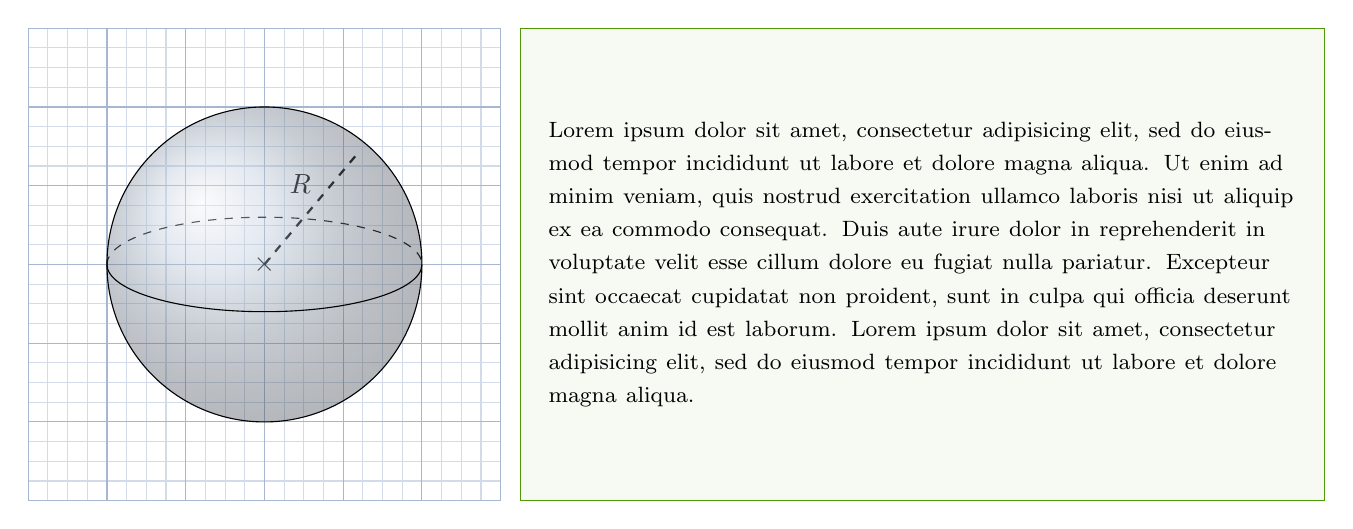
\begin{tikzpicture}[scale=1]
	% Draw the grid.
	\draw [cornflower!20,step=0.25,thin] (-3,-3) grid (3,3);
	\draw [cornflower!40,step=1.0,thin] (-3,-3) grid (3,3);

	% Label the center
	\node at (0,0) [] {$\times$};

	% x and y components for point where radial line intersects surface. The radius
	% of the sphere, drawn below, is 2cm. Set the length of this line to < 2cm, so 
	% it appears to end at a point in the foreground.
    \pgfmathsetmacro\Rx{1.8*cos(50)};
    \pgfmathsetmacro\Ry{1.8*sin(50)};
    \draw [thick, dashed] (0,0)--(\Rx,\Ry);
	% Label the line.
	\node at (\Rx,\Ry) [xshift=-2em, yshift=-1em] {$R$};

 
 	% Draw the background portion of the equator as dashed.
    \draw[dashed] (-2,0) arc (180:0:2cm and 0.6cm);
	% Draw the sphere as a shaded ball.
    \shade[ball color=cornflower!40!white,opacity=0.40] (0,0) circle (2cm);
	% Outline the sphere.
	\draw (0,0) circle (2cm);
 	% Draw the foreground arc of the equator.
	\draw (-2,0) arc (180:360:2cm and 0.6cm);
 	
	\tikzstyle{information text}=[fill=chameleon!5,inner sep=1em,draw=chameleon]
  \draw[xshift=3.25cm] node [right,text width=9.5cm, style=information text, minimum height=6cm]
    {\footnotesize
	 Lorem ipsum dolor sit amet, consectetur adipisicing elit, sed do eiusmod tempor incididunt ut labore et dolore magna aliqua. Ut enim ad minim veniam, quis nostrud exercitation ullamco laboris nisi ut aliquip ex ea commodo consequat. Duis aute irure dolor in reprehenderit in voluptate velit esse cillum dolore eu fugiat nulla pariatur. Excepteur sint occaecat cupidatat non proident, sunt in culpa qui officia deserunt mollit anim id est laborum. Lorem ipsum dolor sit amet, consectetur adipisicing elit, sed do eiusmod tempor incididunt ut labore et dolore magna aliqua.
	};
\end{tikzpicture}	

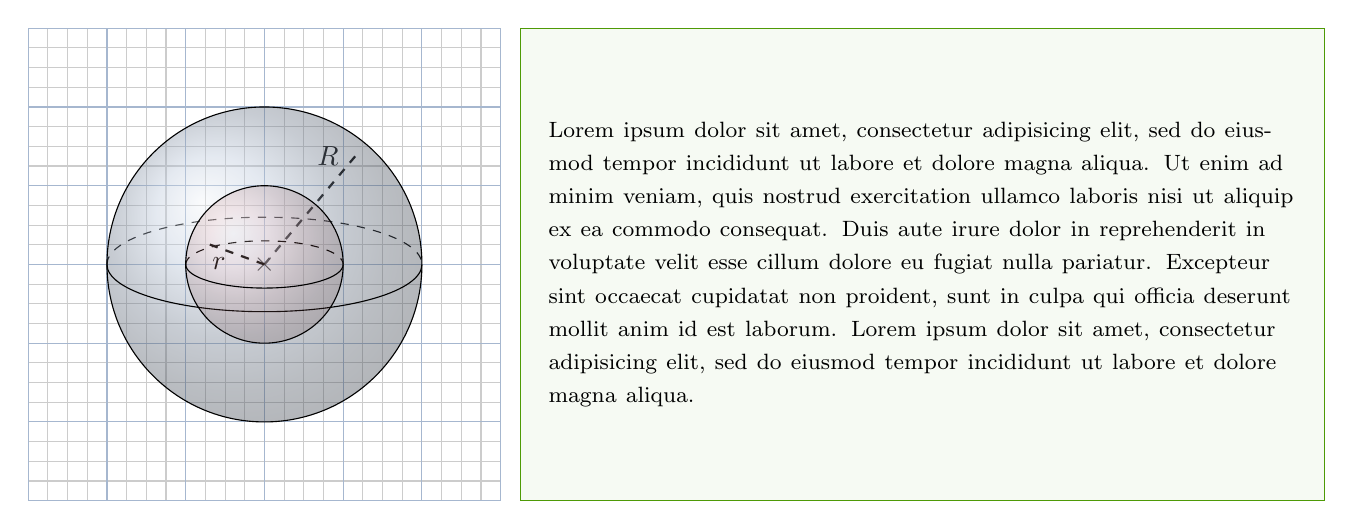
\begin{tikzpicture}[scale=1]
	% Draw the grid.
	\draw [black!20,step=0.25,thin] (-3,-3) grid (3,3);
	\draw [cornflower!40,step=1.0,thin] (-3,-3) grid (3,3);

	\node at (0,0) [] {$\times$};

    \pgfmathsetmacro\Rx{1.8*cos(50)};
    \pgfmathsetmacro\Ry{1.8*sin(50)};
    \draw [thick, dashed] (0,0)--(\Rx,\Ry);
	\node at (\Rx,\Ry) [xshift=-1em, yshift=-0em] {$R$};
 
 
    \draw[dashed] (-2,0) arc (180:0:2cm and 0.6cm);
    \shade[ball color=cornflower!40!white,opacity=0.40] (0,0) circle (2cm);
    \draw (0,0) circle (2cm);
    \draw (-2,0) arc (180:360:2cm and 0.6cm);

	% Set the radius of the Gaussian Sphere.
    \pgfmathsetmacro\Grad{1};
	% Compute x and y coordinates where radial line appears to intersect surface.
    \pgfmathsetmacro\Gx{0.8*\Grad*cos(160)};
    \pgfmathsetmacro\Gy{0.8*\Grad*sin(160)};
    \draw [thick, dashed] (0,0)--(\Gx,\Gy);
	\node at (\Gx,\Gy) [xshift=.5em, yshift=-.75em] {$r$};

	% For drawing equatorial arcs.
    \pgfmathsetmacro\Gcurv{0.3*\Grad};	
    \draw[dashed] (-\Grad,0) arc (180:0:\Grad cm and \Gcurv cm);
    \shade[ball color=scarlet!40!white,opacity=0.20] (0,0) circle (\Grad cm);
    \draw (0,0) circle (\Grad cm);
    \draw (-\Grad,0) arc (180:360:\Grad cm and \Gcurv cm);

	\tikzstyle{information text}=[fill=chameleon!5,inner sep=1em,draw=chameleon]
  \draw[xshift=3.25cm] node [right,text width=9.5cm, style=information text, minimum height=6cm]
    {\footnotesize
	 Lorem ipsum dolor sit amet, consectetur adipisicing elit, sed do eiusmod tempor incididunt ut labore et dolore magna aliqua. Ut enim ad minim veniam, quis nostrud exercitation ullamco laboris nisi ut aliquip ex ea commodo consequat. Duis aute irure dolor in reprehenderit in voluptate velit esse cillum dolore eu fugiat nulla pariatur. Excepteur sint occaecat cupidatat non proident, sunt in culpa qui officia deserunt mollit anim id est laborum. Lorem ipsum dolor sit amet, consectetur adipisicing elit, sed do eiusmod tempor incididunt ut labore et dolore magna aliqua.
	};
\end{tikzpicture}	
  
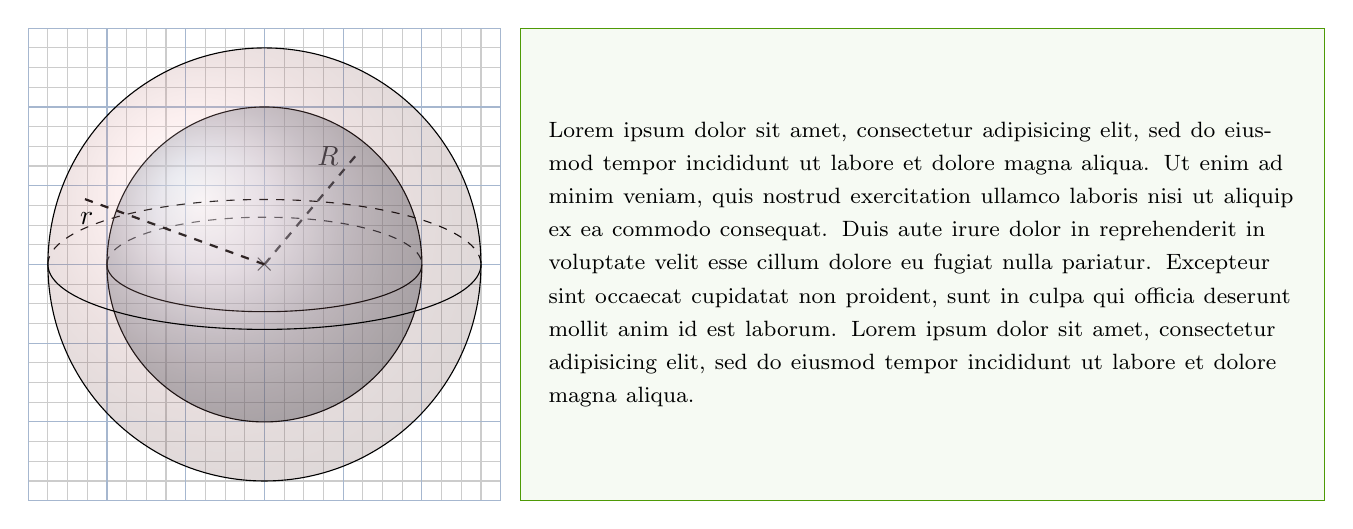
\begin{tikzpicture}[scale=1]
	% Draw the grid.
	\draw [black!20,step=0.25,thin] (-3,-3) grid (3,3);
	\draw [cornflower!40,step=1.0,thin] (-3,-3) grid (3,3);

	\node at (0,0) [] {$\times$};
    \pgfmathsetmacro\Rx{1.8*cos(50)};
    \pgfmathsetmacro\Ry{1.8*sin(50)};
    \draw [thick, dashed] (0,0)--(\Rx,\Ry);
	\node at (\Rx,\Ry) [xshift=-1em, yshift=-0em] {$R$};
 
 
    \draw[dashed] (-2,0) arc (180:0:2cm and 0.6cm);
    \shade[ball color=cornflower!40!white,opacity=0.40] (0,0) circle (2cm);
    \draw (0,0) circle (2cm);
    \draw (-2,0) arc (180:360:2cm and 0.6cm);

    \pgfmathsetmacro\Grad{2.75};
    \pgfmathsetmacro\Gx{0.9*\Grad*cos(160)};
    \pgfmathsetmacro\Gy{0.9*\Grad*sin(160)};
    \pgfmathsetmacro\Gcurv{0.3*\Grad};
    \draw [thick, dashed] (0,0)--(\Gx,\Gy);
	
    \draw[dashed] (-\Grad,0) arc (180:0:\Grad cm and \Gcurv cm);
    \shade[ball color=scarlet!40!white,opacity=0.20] (0,0) circle (\Grad cm);
 	\draw (0,0) circle (\Grad cm);
    \draw (-\Grad,0) arc (180:360:\Grad cm and \Gcurv cm);
 	\node at (\Gx,\Gy) [xshift=.2em, yshift=-.75em] {$r$};

	\tikzstyle{information text}=[fill=chameleon!5,inner sep=1em,draw=chameleon]
  \draw[xshift=3.25cm] node [right,text width=9.5cm, style=information text, minimum height=6cm]
    {\footnotesize
	 Lorem ipsum dolor sit amet, consectetur adipisicing elit, sed do eiusmod tempor incididunt ut labore et dolore magna aliqua. Ut enim ad minim veniam, quis nostrud exercitation ullamco laboris nisi ut aliquip ex ea commodo consequat. Duis aute irure dolor in reprehenderit in voluptate velit esse cillum dolore eu fugiat nulla pariatur. Excepteur sint occaecat cupidatat non proident, sunt in culpa qui officia deserunt mollit anim id est laborum. Lorem ipsum dolor sit amet, consectetur adipisicing elit, sed do eiusmod tempor incididunt ut labore et dolore magna aliqua.
	};

 \end{tikzpicture}	
 
\end{center}



\end{document}